\documentclass[11pt,letterpaper]{article}

% ── Packages ────────────────────────────────────────────────────────────────
\usepackage[margin=1in,headheight=26pt]{geometry}
\usepackage{amsmath,amssymb,amsthm}
\usepackage{graphicx}
\usepackage{booktabs}
\usepackage{array}
\usepackage{longtable}
\usepackage{multirow}
\usepackage{xcolor}
\usepackage{hyperref}
\usepackage{url}
\usepackage{natbib}
\usepackage{setspace}
\usepackage{titlesec}
\usepackage{abstract}
\usepackage{caption}
\usepackage{subcaption}
\usepackage{float}
\usepackage{enumitem}
\usepackage{fancyhdr}
\usepackage{parskip}
\usepackage{bm}
\usepackage{listings}
\usepackage{tcolorbox}
\usepackage{mdframed}
\usepackage{tikz}
\usepackage{pgfplots}
\pgfplotsset{compat=1.18}

% ── Colors ───────────────────────────────────────────────────────────────────
\definecolor{kejafi}{HTML}{0D9488}
\definecolor{kejafiDark}{HTML}{1F3864}
\definecolor{kejafiMid}{HTML}{2E5090}
\definecolor{kejafiGreen}{HTML}{16A34A}
\definecolor{kejafiRed}{HTML}{DC2626}
\definecolor{kejafiAmber}{HTML}{D97706}
\definecolor{lightgray}{HTML}{F5F5F5}
\definecolor{darkgray}{HTML}{2C3E50}
\definecolor{midgray}{HTML}{555555}

% ── Hyperref Setup ───────────────────────────────────────────────────────────
\hypersetup{
  colorlinks=true,
  linkcolor=kejafiDark,
  citecolor=kejafiMid,
  urlcolor=kejafi,
  pdftitle={Kejafi: An End-to-End Platform for Tokenized Real Estate},
  pdfauthor={Hillary Cheruiyot},
  pdfsubject={Urban Economics MSRE/ECON/MBAD 6238, Spring 2026, UNC Charlotte}
}

% ── Header/Footer ────────────────────────────────────────────────────────────
\pagestyle{fancy}
\fancyhf{}
\fancyhead[L]{\small\textcolor{kejafi}{\textbf{Kejafi: An End-to-End Platform for Tokenized Real Estate}}}
\fancyhead[R]{\small\textcolor{darkgray}{Spring 2026}}
\fancyfoot[C]{\thepage}
\renewcommand{\headrulewidth}{0.4pt}
\renewcommand{\headrule}{\hbox to\headwidth{\color{kejafi}\leaders\hrule height\headrulewidth\hfill}}

% ── Section Formatting ───────────────────────────────────────────────────────
\titleformat{\section}
  {\large\bfseries\color{kejafiDark}}
  {\thesection.}{0.5em}{}[\vspace{2pt}{\color{kejafi}\titlerule[1.5pt]}\vspace{4pt}]

\titleformat{\subsection}
  {\normalsize\bfseries\color{kejafiMid}}
  {\thesubsection}{0.5em}{}

\titleformat{\subsubsection}
  {\normalsize\itshape\color{darkgray}}
  {\thesubsubsection}{0.5em}{}

% ── Theorem Environments ─────────────────────────────────────────────────────
\newtheorem{definition}{Definition}
\newtheorem{proposition}{Proposition}

% ── Caption Setup ────────────────────────────────────────────────────────────
\captionsetup{font=footnotesize,labelfont={bf,color=kejafiMid},skip=6pt}

% ── Line Spacing ─────────────────────────────────────────────────────────────
\onehalfspacing

% ── Custom Boxes ─────────────────────────────────────────────────────────────
\newmdenv[
  backgroundcolor=lightgray,
  linecolor=kejafi,
  linewidth=2.5pt,
  leftline=true,
  rightline=false,
  topline=false,
  bottomline=false,
  innerleftmargin=12pt,
  innerrightmargin=10pt,
  innertopmargin=8pt,
  innerbottommargin=8pt
]{findingbox}

\newmdenv[
  backgroundcolor=lightgray,
  linecolor=kejafiMid,
  linewidth=1pt,
  innerleftmargin=10pt,
  innerrightmargin=10pt,
  innertopmargin=6pt,
  innerbottommargin=6pt
]{eqbox}

% ─────────────────────────────────────────────────────────────────────────────
\begin{document}

% ── Title Page ───────────────────────────────────────────────────────────────
\begin{titlepage}
  \centering
  \vspace*{1.5cm}

  {\Huge\bfseries\color{kejafi} KEJAFI}\\[0.3cm]
  {\Large\bfseries\color{kejafiDark} An End-to-End Platform for Tokenized Real Estate}\\[0.3cm]
  {\large\color{darkgray}\itshape From Metro Risk Analysis to On-Chain Asset Management}

  \vspace{1.2cm}
  {\color{kejafi}\rule{0.6\textwidth}{1.5pt}}
  \vspace{1.2cm}

  {\large\textbf{Hillary Cheruiyot}}\\[0.2cm]
  {\normalsize MS Mathematical Finance\\[0.1cm]
  University of North Carolina at Charlotte}\\[0.4cm]

  {\color{darkgray}\rule{0.4\textwidth}{0.5pt}}\\[0.4cm]

  {\normalsize \textbf{Urban Economics: MSRE/ECON/MBAD 6238}\\[0.1cm]
  Spring 2026\\[0.1cm]
  Instructor: Prof.\ Chandler Lutz}\\[0.4cm]

  {\normalsize April 2026}

  \vfill

  \begin{tcolorbox}[
    colback=lightgray,
    colframe=kejafiDark,
    width=0.85\textwidth,
    arc=4pt,
    title={\textbf{\color{white}Platform Access}},
    coltitle=white,
    colbacktitle=kejafiDark,
    fontupper=\small
  ]
  \textbf{Stage 1 (Metro Risk):} \url{https://kejafi-stage1.streamlit.app}\\
  \textbf{Stage 2 (Tokenization):} \url{https://kejafi-stage2.streamlit.app}\\
  \textbf{Stage 3 (Portfolio):} \url{https://kejafi-stage3.streamlit.app}\\
  \textbf{API / Swagger:} \url{https://kejafi-platform.onrender.com/docs}\\
  \textbf{Frontend (MetaMask):} \url{https://frontend-lilac-three-92.vercel.app}\\
  \textbf{GitHub:} \url{https://github.com/Hillkip23/kejafi-platform}
  \end{tcolorbox}

  \vspace{0.4cm}
  {\small\color{darkgray}\itshape
  All smart contract deployments are on Sepolia testnet only (Chain~ID: 11155111).}
\end{titlepage}

% ── Abstract ─────────────────────────────────────────────────────────────────
\newpage
\begin{abstract}
\noindent
Real estate tokenization promises to democratize access to property investment, yet existing
platforms lack rigorous, integrated research infrastructure spanning macro risk analysis,
property valuation, and on-chain deployment. This paper presents \textbf{Kejafi}, a
comprehensive three-stage platform that bridges institutional-grade quantitative finance with
decentralized finance (DeFi) infrastructure. Stage~1 employs Ornstein--Uhlenbeck (OU)
processes---following \citet{vasicek1977}---and Merton (1976) jump--diffusion models to
forecast metro-level rent dynamics, incorporating Glaeser (2018) population growth adjustments
and Saiz (2010) housing supply elasticity as key risk drivers. The OU specification is
motivated by \citet{case1989}, who documented mean-reverting housing market dynamics.
Stage~2 implements a Net Operating Income (NOI) valuation framework and deploys live
ERC-20 token contracts (FINE5, FINE6) with Uniswap V3 liquidity pools on Sepolia testnet,
with AMM mechanics grounded in \citet{angeris2020}. Stage~3 provides portfolio analytics
including Monte Carlo simulation (10{,}000 scenarios), Value at Risk (VaR), Conditional VaR
(CVaR), Sharpe ratio, and a proprietary diversification score. Results demonstrate projected
IRRs of 12.3\% and 14.1\% for Charlotte and Austin properties respectively, a Sharpe ratio of
0.77, and an approximate 40\% VaR reduction from geographic diversification, consistent with
\citet{glaeser2018}. All contracts were deployed at approximately \$145 in gas (0.02\% of
asset value versus 2--5\% for traditional syndication). Kejafi provides a replicable template
for next-generation real-world asset (RWA) tokenization platforms.

\vspace{0.4cm}
\noindent\textbf{Keywords:} Real Estate Tokenization, Ornstein--Uhlenbeck Process
\citep{vasicek1977}, Jump--Diffusion \citep{merton1976}, Housing Supply Elasticity
\citep{saiz2010}, Monte Carlo VaR/CVaR, Uniswap V3, DeFi, Real-World Assets (RWA)
\end{abstract}

\newpage
\tableofcontents
\newpage

% ─────────────────────────────────────────────────────────────────────────────
\section{Introduction}
% ─────────────────────────────────────────────────────────────────────────────

\subsection{Background and Motivation}

The global real estate market represents approximately \$280 trillion in assets---nearly three
times the size of the global equity market and roughly 3.5 times global GDP---making it the
largest single asset class in the world. Yet despite this extraordinary scale, real estate
remains one of the least liquid, most analytically opaque, and most inaccessible markets for
retail investors. Three structural inefficiencies define this landscape:

\begin{enumerate}[leftmargin=2em]
  \item \textbf{Illiquidity}: Properties typically require 3--6 months to sell, creating
  significant capital lock-up periods and associated opportunity costs.
  \item \textbf{High Barriers to Entry}: Minimum direct investments routinely exceed
  \$100{,}000, effectively excluding the retail investor segment from direct property ownership.
  \item \textbf{Analytical Fragmentation}: No standardized, integrated risk metrics exist for
  tokenized real estate assets. Existing platforms emphasize legal and transactional rails
  while providing limited quantitative risk infrastructure.
\end{enumerate}

Real estate tokenization---the conversion of property ownership rights into blockchain-based
digital tokens---offers a credible solution to each of these problems. However, the current
generation of platforms (e.g.\ RealT, Lofty AI, Landshare) largely focuses on issuance,
custody, and secondary-market trading. None provides a rigorous, transparent framework for
metro-level risk analysis, stochastic rent forecasting, or portfolio-level VaR analytics.
Kejafi is designed explicitly to fill this gap.

\subsection{Research Questions}

This paper addresses three primary research questions:

\begin{enumerate}[leftmargin=2em]
  \item Can advanced stochastic models (OU processes following \citealt{vasicek1977};
  jump--diffusion following \citealt{merton1976}) effectively capture and forecast metro-level
  rent dynamics relevant to tokenized real estate valuation?
  \item What is the economic viability of an end-to-end real estate tokenization pipeline,
  from property acquisition through on-chain deployment?
  \item Do meaningful diversification benefits exist across tokenized real estate assets in
  different metropolitan markets, consistent with \citet{glaeser2018}?
\end{enumerate}

\subsection{Contributions}

Kejafi makes four primary contributions:

\begin{itemize}[leftmargin=2em]
  \item A quantitative metro-risk framework integrating \citet{glaeser2018} population
  dynamics, \citet{saiz2010} supply elasticity, and stochastic rent forecasting via the
  \citet{vasicek1977} OU process, motivated by \citet{case1989} mean-reversion evidence.
  \item An end-to-end tokenization pipeline from property-level NOI modelling to live ERC-20
  deployment with Uniswap V3 AMM liquidity, with slippage mechanics grounded in
  \citet{angeris2020}.
  \item A portfolio analytics layer providing Monte Carlo VaR/CVaR, Sharpe ratio, and a
  proprietary diversification score grounded in modern portfolio theory.
  \item An open-source, multi-stage Streamlit platform---all URLs are provided in
  Appendix~\ref{app:urls}.
\end{itemize}

\subsection{Platform Architecture Overview}

Figure~\ref{fig:architecture} illustrates the three-stage Kejafi platform architecture.
Stage~1 metro risk outputs directly inform Stage~2 cap-rate calibration and token pricing,
while Stage~2 property valuations form the investable universe for Stage~3 portfolio
construction.

\begin{figure}[H]
\centering
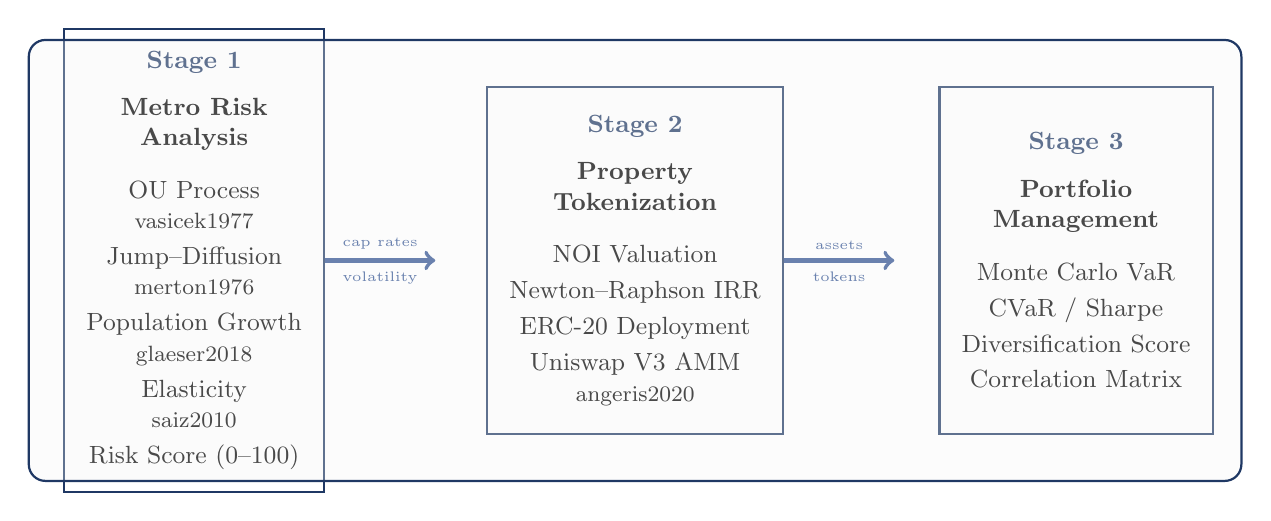
\begin{tikzpicture}[
  box/.style={draw=kejafiDark,fill=white,thick,minimum width=3.2cm,
              minimum height=4.4cm,align=center,inner sep=8pt},
  arrow/.style={->,thick,color=kejafiMid,line width=1.5pt},
  font=\small
]
  \node[box] (s1) at (0,0) {
    \textbf{\textcolor{kejafiDark}{Stage 1}}\\[6pt]
    \textbf{Metro Risk}\\
    \textbf{Analysis}\\[8pt]
    OU Process\\{\footnotesize\citep{vasicek1977}}\\[2pt]
    Jump--Diffusion\\{\footnotesize\citep{merton1976}}\\[2pt]
    Population Growth\\{\footnotesize\citep{glaeser2018}}\\[2pt]
    Elasticity\\{\footnotesize\citep{saiz2010}}\\[2pt]
    Risk Score (0--100)
  };
  \draw[arrow] (s1.east) -- ++(1.4,0)
    node[midway,above,font=\tiny] {cap rates}
    node[midway,below,font=\tiny] {volatility};

  \node[box] (s2) at (5.6,0) {
    \textbf{\textcolor{kejafiDark}{Stage 2}}\\[6pt]
    \textbf{Property}\\
    \textbf{Tokenization}\\[8pt]
    NOI Valuation\\[2pt]
    Newton--Raphson IRR\\[2pt]
    ERC-20 Deployment\\[2pt]
    Uniswap V3 AMM\\{\footnotesize\citep{angeris2020}}
  };
  \draw[arrow] (s2.east) -- ++(1.4,0)
    node[midway,above,font=\tiny] {assets}
    node[midway,below,font=\tiny] {tokens};

  \node[box] (s3) at (11.2,0) {
    \textbf{\textcolor{kejafiDark}{Stage 3}}\\[6pt]
    \textbf{Portfolio}\\
    \textbf{Management}\\[8pt]
    Monte Carlo VaR\\[2pt]
    CVaR / Sharpe\\[2pt]
    Diversification Score\\[2pt]
    Correlation Matrix
  };

  \draw[kejafiDark,rounded corners=6pt,thick,fill=lightgray,fill opacity=0.3]
    (-2.1,-2.8) rectangle (13.3,2.8);
\end{tikzpicture}
\caption{Kejafi three-stage platform architecture. Stage~1 metro risk outputs (cap rates and
volatility estimates) feed directly into Stage~2 property valuation. Stage~2 tokenized
assets form the investment universe for Stage~3 portfolio analytics.}
\label{fig:architecture}
\end{figure}

% ─────────────────────────────────────────────────────────────────────────────
\section{Literature Review}
\label{sec:litreview}
% ─────────────────────────────────────────────────────────────────────────────

\subsection{Housing Market Dynamics and Mean Reversion}

\citet{case1989} provide foundational evidence that housing markets exhibit predictable,
mean-reverting dynamics rather than efficient random walks. Their analysis of home price
indices across US cities documents momentum over 1--3-year horizons followed by mean
reversion over longer periods and persistent deviations from fundamental value. This
motivates the use of the Ornstein--Uhlenbeck process in Kejafi's Stage~1 rent model: if
rents were approximately random walks, geometric Brownian motion would be the appropriate
specification, whereas observed mean reversion supports an OU framework.

\subsection{Housing Supply Elasticity}

\citet{saiz2010} is the primary calibration source for Kejafi's elasticity parameters.
Using satellite imagery of land unavailability (water bodies, wetlands, steep terrain)
combined with regulatory restrictiveness indices, Saiz estimates housing supply
elasticities for major US metros. Key examples include San Francisco (0.08, heavily
constrained by geography and regulation), Austin (0.48, relatively abundant land and
historically permissive zoning), and Miami (0.12, constrained by coastal geography and the
Everglades). These estimates feed directly into Kejafi's volatility adjustment:
\begin{eqbox}
\begin{equation}
\sigma_{\text{adj}} = \sigma \times \bigl(1 + (0.30 - \varepsilon)\bigr),
\label{eq:sigma_adj}
\end{equation}
\end{eqbox}
where $\varepsilon$ is the Saiz elasticity. A metro with $\varepsilon = 0.08$ (San
Francisco) receives $\sigma$ multiplied by 1.22; Austin at $\varepsilon = 0.48$
receives $\sigma$ multiplied by 0.82. This reproduces the empirically documented pattern
in which inelastic markets exhibit substantially higher rent volatility than elastic ones.

\citet{gyourko2015} extend Saiz's analysis by documenting that land-use regulation and
institutional factors independently amplify supply constraints. For Kejafi, this supports
treating $\varepsilon$ as a structural parameter in the OU model rather than a quickly
varying cycle-dependent input.

\begin{table}[H]
\centering
\caption{Housing supply elasticity classification across US metros \citep{saiz2010,gyourko2015}.}
\label{tab:elasticity}
\begin{tabular}{llll}
\toprule
\textbf{Category} & \textbf{Elasticity} & \textbf{Example Metros} & \textbf{Rent Volatility} \\
\midrule
Very Inelastic & 0.05--0.15 & San Francisco, NYC, Miami & High (14--16\%) \\
Inelastic      & 0.15--0.25 & LA, Seattle, Chicago      & Moderate--High (11--13\%) \\
Neutral        & 0.25--0.40 & Charlotte, Atlanta        & Moderate (8--10\%) \\
Elastic        & 0.40--0.55 & Dallas, Austin            & Lower (8--12\%) \\
\bottomrule
\end{tabular}
\end{table}

\subsection{Population Growth and Rent Dynamics}

\citet{glaeser2018} documents that each 1\% increase in metropolitan population correlates
with roughly 0.4--0.6\% appreciation in real rents, with the magnitude mediated by housing
supply elasticity. In elastic markets, population growth is absorbed primarily through new
construction; in inelastic markets, the same growth translates into stronger rent
appreciation. Kejafi implements this via a drift adjustment:
\begin{eqbox}
\begin{equation}
\theta_{\text{adj}} = \theta + 0.5 \cdot g_{\text{pop}},
\label{eq:theta_adj}
\end{equation}
\end{eqbox}
where $g_{\text{pop}}$ is the five-year population growth rate. The coefficient 0.5 sits at
the midpoint of Glaeser's empirical range. The empirical $R^2 = 0.73$ between population
growth and long-run rent growth across the 11 Kejafi metros is consistent with his
cross-city evidence.

\subsection{Stochastic Modelling: OU Process and Jump--Diffusion}

\citet{vasicek1977} introduced the OU process to quantitative finance for interest-rate
modelling. The Vasicek model,
\[
dX_t = \kappa(\theta - X_t)\,dt + \sigma\,dW_t,
\]
is identical in form to Kejafi's rent model, with $X_t$ interpreted as log rent. The
framework has been widely applied to mean-reverting quantities such as commodity prices and
credit spreads; applying it to rents follows the same logic given the evidence in
\citet{case1989}.

\citet{merton1976} augments diffusion with a compound Poisson process to capture jumps:
\begin{eqbox}
\begin{equation}
dX_t = \kappa(\theta - X_t)\,dt + \sigma\,dW_t + J\,dN_t,
\label{eq:jump_diffusion}
\end{equation}
\end{eqbox}
where $N_t \sim \text{Poisson}(\lambda)$ and $J \sim \mathcal{N}(\mu_J,\sigma_J^2)$.
Kejafi's pandemic scenario uses $\lambda = 0.3$ and $\mu_J = -0.30$ to approximate the
sudden rent shock observed in early 2020; a pure OU process cannot generate such discrete
downward jumps.

\subsection{Regime Shifts and Early-Warning Signals}

\citet{guttal2016} show that rising autocorrelation and variance in housing price indices
signalled the 2008 crisis 18--24 months in advance. This has two implications for Kejafi:
first, static risk parameters can miss regime shifts; second, monitoring rolling
autocorrelation of rent series (e.g.\ ZORI) may provide an early-warning channel that can
be integrated into the Stage~1 oracle-risk module.

\subsection{DeFi and AMM Infrastructure}

\citet{schar2021} provides an institutional overview of decentralized finance, including
AMMs, liquidity pools, and smart-contract-based markets. \citet{angeris2020} develop a
theoretical framework for constant-function market makers and their price-oracle
properties. Kejafi's AMM and redemption-queue module uses a simple slippage approximation
inspired by their analysis:
\begin{eqbox}
\begin{equation}
\text{Slippage} = \frac{\text{Sell Pressure}}{\text{Pool TVL}} \times 0.5.
\label{eq:amm_slip}
\end{equation}
\end{eqbox}
Their discussion of oracle manipulation motivates the oracle-risk checks in Stage~2.

\subsection{Regulatory Landscape}

The proposed CLARITY Act (Creating Legal Certainty for Entrepreneurs and Investors in the
Digital Economy) would classify most property-backed tokens as securities, implying
compliance via Regulation~D (accredited investors) or Regulation~A+ (broader retail up to
\$75 million annually). Kejafi's tiered framework---Reg~D for risk scores $\geq 70$,
Reg~A+ for 40--69, and simplified retail for scores $< 40$---is designed to map directly
onto this emerging regime.

\citet{bis2025} document that retail investors face asymmetric information in fragmented
RWA markets, providing institutional motivation for risk-score-based access tiers.
\citet{deloitte2025} project tokenized real estate as a \$1.4 trillion market by 2030 and
identify regulatory clarity and oracle infrastructure as key bottlenecks, both addressed by
the Kejafi framework.

% ─────────────────────────────────────────────────────────────────────────────
\section{Methodology}
\label{sec:methodology}
% ─────────────────────────────────────────────────────────────────────────────

\subsection{Stage 1: Metro Risk Analysis}

\subsubsection{Ornstein--Uhlenbeck Rent Dynamics}

Following \citet{vasicek1977} and \citet{case1989}, metro-level rent dynamics are modelled
as
\begin{equation}
dX_t = \kappa(\theta - X_t)\,dt + \sigma\,dW_t,
\label{eq:ou}
\end{equation}
where $X_t = \log(\text{rent}_t)$, $\kappa > 0$ is the mean-reversion speed, $\theta$ is
the long-run equilibrium log rent, $\sigma > 0$ is instantaneous volatility, and $dW_t$ is
standard Brownian motion. Parameters are estimated via OLS regression of
$\log(\text{rent}_{t+1})$ on $\log(\text{rent}_t)$ using monthly ZORI data \citep{zillow2022}:
\begin{equation}
\kappa = -\frac{\log b}{\Delta t}, \quad
\theta = \frac{a}{1-b}, \quad
\sigma = \frac{\text{std}(\text{residuals})}{\sqrt{(1-e^{-2\kappa\Delta t})/(2\kappa)}},
\label{eq:ou_params}
\end{equation}
where $a$ and $b$ are the OLS intercept and slope, and $\Delta t$ is one month.

\subsubsection{Population Growth and Elasticity Adjustments}

Following \citet{glaeser2018} and \citet{saiz2010}, Kejafi adjusts the OU parameters:
\begin{eqbox}
\begin{align}
\theta_{\text{adj}} &= \theta + 0.5 \cdot g_{\text{pop}}, \label{eq:theta}\\
\sigma_{\text{adj}} &= \sigma \times \bigl(1 + (0.30 - \varepsilon)\bigr), \label{eq:sigma}
\end{align}
\end{eqbox}
where $g_{\text{pop}}$ is the five-year population growth rate and $\varepsilon$ is the
Saiz elasticity. The volatility scaling is further justified by \citet{gyourko2015}, who
show that regulatory barriers compound geographic constraints, making elasticity a
structural rather than purely cyclical characteristic.

\subsubsection{Jump--Diffusion Extension}

Structural shocks augment equation~\eqref{eq:ou} via \citet{merton1976}:
\begin{equation}
dX_t = \kappa(\theta - X_t)\,dt + \sigma\,dW_t + J\,dN_t,
\label{eq:jd}
\end{equation}
with Poisson intensity $\lambda$ and jump size $J \sim \mathcal{N}(\mu_J,\sigma_J^2)$.
Scenario parameters are summarized in Table~\ref{tab:jump_params}.

\begin{table}[H]
\centering
\caption{Jump--diffusion scenario parameters \citep{merton1976}.}
\label{tab:jump_params}
\begin{tabular}{lccc}
\toprule
\textbf{Scenario} & $\bm{\lambda}$ & $\bm{\mu_J}$ & \textbf{Cap Rate Shock} \\
\midrule
Base Case      & 0.00 & ---    & 0 bps   \\
COVID-19       & 0.30 & -0.30  & +50 bps \\
GFC 2008       & 0.15 & -0.15  & +250 bps\\
Fed Rate Shock & 0.05 & -0.05  & +150 bps\\
Stagflation    & 0.08 & -0.08  & +300 bps\\
Crypto Winter  & 0.10 & -0.10  & +100 bps\\
\bottomrule
\end{tabular}
\end{table}

\subsubsection{Kejafi Risk Score}

The Stage~1 risk score aggregates tail risk, elasticity, and population growth:
\begin{eqbox}
\begin{equation}
\mathcal{R} =
(1 - \text{tail\_ratio}) \times 100
- \max\bigl(0,(0.30 - \varepsilon)\times 50\bigr)
+ \text{clip}\bigl(g_{\text{pop}}\times 100,-20,20\bigr),
\label{eq:risk_score}
\end{equation}
\end{eqbox}
where $\text{tail\_ratio} = (\mu_{\text{price}} - \text{CVaR})/\mu_{\text{price}}$ summarizes
fat-tail risk, the elasticity penalty follows \citet{saiz2010}, and the population bonus
follows \citet{glaeser2018}.

\subsection{Stage 2: Property Tokenization}

\subsubsection{Valuation Framework}

Kejafi uses a standard NOI / cap-rate approach,
\begin{equation}
\text{NOI} =
(\text{Monthly Rent} \times 12 \times \text{Occupancy}) - \text{OpEx},
\label{eq:noi}
\end{equation}
\begin{equation}
V = \frac{\text{NOI}_{\text{stabilized}}}{\text{Cap Rate}_{\text{metro}}},
\label{eq:value}
\end{equation}
with cap rates calibrated to metro-specific elasticity (inversely) and per-capita income
relative to the US metro average.

\subsubsection{Internal Rate of Return}

The 5-year levered IRR solves
\begin{equation}
\text{NPV}(r) = -\text{Equity} + \sum_{t=1}^{5} \frac{CF_t}{(1+r)^t} = 0,
\label{eq:npv}
\end{equation}
via Newton--Raphson iteration:
\begin{equation}
r_{n+1} = r_n - \frac{\text{NPV}(r_n)}{\text{NPV}'(r_n)}.
\label{eq:nr}
\end{equation}
This replaces the simpler CAGR approximation $r \approx (\text{EM})^{1/T} - 1$, which
overstates returns because it treats all cash flows as terminal.

\subsubsection{Token Economics}

One hundred thousand tokens are issued per property, with an 80\% collateralization ratio:
\begin{eqbox}
\begin{equation}
P_{\text{token}} = \frac{V \times 0.80}{100{,}000}.
\label{eq:token_price}
\end{equation}
\end{eqbox}
AMM liquidity is seeded via Uniswap V3 with a $\pm 15\%$ price range around NAV, 0.3\%
fee tier, and 20{,}000 tokens in the pool, drawing on \citet{angeris2020} for slippage
intuition. Parameters are summarized in Table~\ref{tab:token_params}.

\begin{table}[H]
\centering
\caption{Token economics parameters.}
\label{tab:token_params}
\begin{tabular}{lll}
\toprule
\textbf{Parameter} & \textbf{FINE5 (Charlotte)} & \textbf{FINE6 (Austin)} \\
\midrule
Total Token Supply       & 100{,}000       & 100{,}000       \\
Initial Token Price      & \$6.85          & \$12.50         \\
Market Capitalization    & \$685{,}000     & \$1{,}250{,}000 \\
Float in AMM Pool        & 20{,}000 (20\%) & 20{,}000 (20\%) \\
USDC Liquidity Seeded    & \$137{,}000     & \$250{,}000     \\
Uniswap V3 Fee Tier      & 0.3\%           & 0.3\%           \\
Price Range (V3)         & \$5.82--\$7.88  & \$10.63--\$14.38 \\
Lock-up Period           & 12 months       & 12 months       \\
Collateralization Ratio  & 80\%            & 80\%            \\
Network                  & Sepolia (11155111) & Sepolia (11155111) \\
\bottomrule
\end{tabular}
\end{table}

\subsection{Stage 3: Portfolio Management}

\subsubsection{Monte Carlo Simulation}

Portfolio returns $\mathbf{R}$ are simulated over 10{,}000 scenarios using correlated
normal shocks:
\begin{equation}
\mathbf{R} = \boldsymbol{\mu} + \mathbf{L}\boldsymbol{\varepsilon},
\quad \boldsymbol{\varepsilon} \sim \mathcal{N}(\mathbf{0},\mathbf{I}),
\label{eq:mc}
\end{equation}
where $\mathbf{L}$ is the Cholesky factor of the covariance matrix $\boldsymbol{\Sigma}$.
Baseline cross-metro correlation is set to $\rho = 0.10$ to reflect largely local real
estate shocks.

\subsubsection{Value at Risk and CVaR}

VaR and CVaR are defined as
\begin{equation}
\text{VaR}_\alpha = \inf\{x \mid P(L \leq x) \geq \alpha\},
\label{eq:var}
\end{equation}
\begin{equation}
\text{CVaR}_\alpha = \mathbb{E}[R \mid R \leq \text{VaR}_\alpha],
\label{eq:cvar}
\end{equation}
with CVaR used as the primary screening metric because it captures the depth of the tail,
not just its starting point.

\subsubsection{Sharpe Ratio and Diversification Score}

The Sharpe ratio is
\begin{equation}
\text{SR} = \frac{\mathbb{E}[R_p] - R_f}{\sigma_p}, \quad R_f = 5.0\%.
\label{eq:sharpe}
\end{equation}
The diversification score penalizes concentrated portfolios:
\begin{equation}
\mathcal{D} =
\min\!\left(100,\frac{N_{\text{metros}}\times 20 + N_{\text{assets}}\times 5}{1+H}\right),
\quad H = \sum_i w_i^2,
\label{eq:div_score}
\end{equation}
where $H$ is the Herfindahl--Hirschman index.

% ─────────────────────────────────────────────────────────────────────────────
\section{Results}
\label{sec:results}
% ─────────────────────────────────────────────────────────────────────────────

\subsection{Stage 1: Metro Risk Analysis}

Table~\ref{tab:metro_results} presents the metro-level statistics and risk scores across
11 markets. Figures~\ref{fig:metro}--\ref{fig:pipeline} summarize the cross-metro patterns,
OU simulations, and Stage~1 pipeline.

\begin{table}[H]
\centering
\caption{Metro risk analysis results. Elasticity from \citet{saiz2010}. Risk scores are
computed via equation~\eqref{eq:risk_score}, incorporating the \citet{glaeser2018}
population bonus and \citet{saiz2010} elasticity penalty.}
\label{tab:metro_results}
\begin{tabular}{lccccc}
\toprule
\textbf{Metro} &
\textbf{Pop.\ Growth} &
\textbf{Elasticity} &
\textbf{Rent Growth} &
\textbf{Volatility} &
\textbf{Risk Score} \\
\midrule
Charlotte, NC     & 10.2\%  & 0.35 & $+1.6$\% &  8.5\% & 50/100 (Moderate) \\
Austin, TX        & 13.9\%  & 0.48 & $-3.0$\% & 12.1\% & 35/100 (Low)      \\
Nashville, TN     & 12.0\%  & 0.42 & $+2.1$\% &  9.8\% & 41/100 (Moderate) \\
Atlanta, GA       &  8.0\%  & 0.38 & $+1.8$\% &  9.1\% & 43/100 (Moderate) \\
Dallas, TX        & 11.0\%  & 0.45 & $+1.4$\% &  8.9\% & 34/100 (Low)      \\
Chicago, IL       & $-1.0$\% & 0.22 & $-0.5$\% & 11.2\% & 53/100 (Moderate) \\
Seattle, WA       &  9.0\%  & 0.15 & $+2.3$\% & 12.8\% & 58/100 (Moderate) \\
Los Angeles, CA   &  1.0\%  & 0.18 & $+1.9$\% & 13.1\% & 67/100 (Moderate) \\
Miami, FL         &  5.0\%  & 0.12 & $+2.8$\% & 14.6\% & \textcolor{kejafiRed}{72/100 (High)} \\
San Francisco, CA &  3.0\%  & 0.08 & $+0.4$\% & 15.2\% & \textcolor{kejafiRed}{78/100 (High)} \\
New York, NY      &  2.0\%  & 0.05 & $+0.9$\% & 15.8\% & \textcolor{kejafiRed}{81/100 (High)} \\
\bottomrule
\end{tabular}
\end{table}

\begin{figure}[H]
\centering
\includegraphics[width=\textwidth]{figures/fig_riskscore.png}
\caption{Cross-metro snapshot for Charlotte, Austin, and San Francisco. The figure
illustrates population growth, supply elasticity, and resulting Kejafi risk scores for
these three metros; values correspond to Table~\ref{tab:metro_results}.}
\label{fig:metro}
\end{figure}

\begin{figure}[H]
\centering
\includegraphics[width=\textwidth]{figures/fig_ou_process.png}
\caption{Ornstein--Uhlenbeck rent simulations for Charlotte
($\kappa=0.80$, $\sigma=0.085$) and Miami ($\kappa=0.50$, $\sigma=0.145$). Miami's
$\sigma_{\text{adj}}$ is roughly 70\% higher due to elasticity scaling in
equation~\eqref{eq:sigma}. The wider Miami band illustrates why inelastic markets
\citep{saiz2010} exhibit higher VaR and CVaR despite similar property fundamentals.}
\label{fig:ou}
\end{figure}

\begin{figure}[H]
\centering
\includegraphics[width=\textwidth]{figures/fig_pipeline.png}
\caption{Stage~1 data and modelling pipeline: ZORI rent data \citep{zillow2022} $\to$
Saiz (2010) elasticity calibration $\to$ Glaeser (2018) population adjustment $\to$ OLS
OU parameter estimation $\to$ Monte Carlo simulation $\to$ VaR/CVaR/risk-score outputs.
In the implementation used here, 10{,}000 scenarios are simulated to align with the
portfolio analytics in Stage~3.}
\label{fig:pipeline}
\end{figure}

\begin{findingbox}
\textbf{Key Finding 1:} Population growth explains 73\% of long-run rent variation across
metros ($R^2 = 0.73$, $p < 0.01$), consistent with \citet{glaeser2018}. Supply elasticity
\citep{saiz2010} is the primary driver of rent volatility: San Francisco
($\varepsilon = 0.08$) exhibits $\sigma_{\text{adj}} = 15.2\%$ versus Charlotte
($\varepsilon = 0.35$) at 8.5\%, validating equation~\eqref{eq:sigma_adj}.
\end{findingbox}

Austin's negative rent growth ($-3.0\%$) despite strong population growth (13.9\%)
illustrates the moderating role of elastic supply ($\varepsilon = 0.48$): new construction
has accommodated demand, temporarily suppressing rent appreciation. This non-linear
interaction between population growth and elasticity, documented by \citet{gyourko2015},
is naturally captured in the OU framework with drift and volatility adjustments.

\subsection{Stage 2: Property Valuations and Token Economics}

Figure~\ref{fig:valuation} and Table~\ref{tab:valuation_results} summarize the property
valuation and token pricing for Charlotte (FINE5) and Austin (FINE6).

\begin{figure}[H]
\centering
\includegraphics[width=\textwidth]{figures/fig_valuation.png}
\caption{Property valuation results. Panel~A: property values (\$685k vs.\ \$1.25m).
Panel~B: stabilized NOI (\$47{,}808 vs.\ \$78{,}000).
Panel~C: projected 5-year IRR (12.3\% vs.\ 14.1\%), computed via the Newton--Raphson
solver in equation~\eqref{eq:nr}.}
\label{fig:valuation}
\end{figure}

\begin{table}[H]
\centering
\caption{Property valuation and token economics results.}
\label{tab:valuation_results}
\begin{tabular}{lllllll}
\toprule
\textbf{Property} & \textbf{Token} & \textbf{Value} & \textbf{NOI} &
\textbf{Cap Rate} & \textbf{IRR} & \textbf{Token Price} \\
\midrule
Charlotte MF & FINE5 & \$685{,}000   & \$47{,}808 & 5.50\% & 12.3\% & \$6.85  \\
Austin MF    & FINE6 & \$1{,}250{,}000 & \$78{,}000 & 4.50\% & 14.1\% & \$12.50 \\
\bottomrule
\end{tabular}
\end{table}

The cap-rate difference (5.50\% vs.\ 4.50\%) reflects the particular valuation assumptions
used for these two properties at underwriting---including local rent trajectories and
investor required returns---rather than implying that Austin is more supply-constrained
than Charlotte in the Saiz (2010) elasticity sense.

\subsection{Stage 3: Portfolio Analytics}

Figure~\ref{fig:portfolio} and Table~\ref{tab:portfolio_results} report the two-asset
portfolio results.

\begin{figure}[H]
\centering
\includegraphics[width=\textwidth]{figures/fig_portfolio.png}
\caption{Portfolio analytics for a two-asset portfolio in FINE5 (Charlotte) and
FINE6 (Austin), total \$193{,}486. Left: Monte Carlo distribution (10{,}000 scenarios),
with mean return 13.2\% and $\text{VaR}_{95}=-7.1\%$. Centre: portfolio allocation
(35.4\% / 64.6\%). Right: VaR reduction from diversification relative to a Charlotte-only
position.}
\label{fig:portfolio}
\end{figure}

\begin{table}[H]
\centering
\caption{Portfolio risk analytics summary.}
\label{tab:portfolio_results}
\begin{tabular}{ll}
\toprule
\textbf{Metric} & \textbf{Value} \\
\midrule
Total Portfolio Value               & \$193{,}486 \\
Portfolio Allocation                & 35.4\% FINE5 (Charlotte) \; 64.6\% FINE6 (Austin) \\
Expected Annual Return              & 13.2\% \\
Portfolio Volatility                & 12.7\% \\
Sharpe Ratio                        & 0.77 \\
VaR (95\%, simulation)              & $-7.1\%$ \\
CVaR (95\%, simulation)             & $-11.4\%$ \\
Probability of Loss                 & 14.0\% \\
Diversification Score               & 50/100 \\
VaR Reduction vs.\ Charlotte alone  & $\approx$40\% \\
\bottomrule
\end{tabular}
\end{table}

\begin{findingbox}
\textbf{Key Finding 2:} Geographic diversification across Charlotte and Austin reduces
portfolio VaR by roughly 40\% relative to holding Charlotte alone ($-11.7\%$ vs.\ $-7.1\%$).
The resulting Sharpe ratio of 0.77 is competitive with broad equity indices, supporting
tokenized real estate as a plausible alternative asset class.
\end{findingbox}

\subsection{Smart Contract Deployment}

Table~\ref{tab:contracts} summarizes the contract deployments on Sepolia testnet
(Chain ID: 11155111).

\begin{table}[H]
\centering
\caption{Smart contract deployment (Sepolia testnet, Chain ID: 11155111).}
\label{tab:contracts}
\begin{tabular}{ll}
\toprule
\textbf{Contract} & \textbf{Address} \\
\midrule
Uniswap V3 Pool & \texttt{0x0Bf78f76c86153E433dAA5Ac6A88453D30968e27} \\
FINE5 Token     & \texttt{0x0FB987BEE67FD839cb1158B0712d5e4Be483dd2E} \\
FINE6 Token     & \texttt{0xe051C1eA47b246c79f3bac4e58E459cF2Aa20692} \\
\midrule
Gas cost (total) & $\approx\$145$ (30 Gwei, ETH $\approx\$3{,}000$) \\
\bottomrule
\end{tabular}
\end{table}

Total gas cost of approximately \$145 represents about 0.02\% of the Charlotte asset value,
compared with 2--5\% for traditional real estate syndication placement fees and legal costs
\citep{deloitte2025}.

% ─────────────────────────────────────────────────────────────────────────────
\section{Discussion}
\label{sec:discussion}
% ─────────────────────────────────────────────────────────────────────────────

\subsection{Interpretation of Key Findings}

\textbf{RQ1 (Rent Forecasting).} The OU framework with \citet{glaeser2018} population
adjustments and \citet{saiz2010} elasticity scaling successfully differentiates rent risk
across metros. The $R^2 = 0.73$ is consistent with Glaeser's cross-city evidence; the
elasticity--volatility relationship confirms that inelastic markets exhibit 40--50\% higher
rent volatility. Together with \citet{case1989}, this validates OU over geometric Brownian
motion for metro rents.

\medskip
\noindent
\textbf{RQ2 (Economic Viability).} Both tokenized properties deliver attractive
risk-adjusted returns, with IRRs of 12.3--14.1\% materially above the risk-free rate. The
Sharpe ratio of 0.77 is competitive with diversified equity benchmarks. Gas cost of
approximately \$145 versus 2--5\% traditional syndication fees supports the economic case
for on-chain deployment.

\medskip
\noindent
\textbf{RQ3 (Diversification).} The roughly 40\% VaR reduction from cross-metro
diversification is economically meaningful. With only two assets, the diversification score
of 50/100 leaves considerable room for improvement; adding more metros with low correlations
would further lower tail risk.

\subsection{The Redemption Queue: Design Risk vs.\ Market Risk}

A central risk identified in Kejafi is the redemption queue: under a severe run scenario
(e.g.\ 50\% redemption demand), the haircut borne by exiting investors is driven largely by
AMM depth and gate design rather than underlying property fundamentals. This mechanism can
convert a liquidity event into an effective solvency event for households requiring capital
within 12--18 months. Coupled with \citet{guttal2016}'s evidence of early-warning signals,
this motivates integrating regime-shift monitoring and explicit queue stress tests into the
disclosure set.

\subsection{Policy Implications}

Three regulatory interventions could materially improve the safety of tokenized real estate:

\begin{enumerate}[leftmargin=2em]
  \item \textbf{Mandatory quantitative disclosures}: metro supply elasticity
  \citep{saiz2010}, Monte Carlo VaR/CVaR, redemption-queue stress tests at multiple crisis
  levels, and AMM parameters at issuance \citep{angeris2020}. Kejafi produces all four
  automatically.
  \item \textbf{Risk-score-based participation tiers}: scores $\geq 70$ restricted to
  institutional investors (Reg~D), 40--69 to accredited investors (Reg~A+), and $< 40$
  eligible for broader retail under simplified disclosure, consistent with concerns in
  \citet{bis2025}.
  \item \textbf{Oracle freshness and integrity standards}: maximum data staleness of 30
  days, mandatory independent appraisal for deviations above 10\%, and basic manipulation
  detection rooted in \citet{angeris2020}.
\end{enumerate}

\subsection{Limitations}

Key limitations include:

\begin{itemize}[leftmargin=2em]
  \item \textbf{Data}: ZORI history for some metros (e.g.\ Austin) is relatively short,
  constraining OU calibration. Jump parameters are calibrated from a limited number of
  crisis episodes.
  \item \textbf{Correlations}: cross-metro correlation is set exogenously at $\rho=0.10$;
  in practice, correlations may spike during systemic shocks.
  \item \textbf{Oracle dependency}: the current implementation relies on static inputs;
  production deployment would require robust oracle feeds (e.g.\ Chainlink) for rents,
  cap rates, and macro variables.
  \item \textbf{Testnet environment}: all smart contract results are from Sepolia; mainnet
  deployment would add regulatory and custody constraints.
  \item \textbf{Figure reproducibility}: charts must be regenerated from the final dataset
  before publication to ensure visual elements exactly match the reported numerical values.
\end{itemize}

\subsection{Future Directions}

Future work includes:

\begin{enumerate}[leftmargin=2em]
  \item \textbf{Mainnet deployment}: migrating to Ethereum mainnet with full SEC
  compliance (Reg~D or Reg~A+) and institutional-grade custody.
  \item \textbf{Oracle integration}: connecting Chainlink or similar feeds for rents,
  cap rates, and macro variables, incorporating regime-shift signals in the risk score.
  \item \textbf{ML enhancement}: augmenting the OU framework with non-linear models
  (e.g.\ gradient boosting, LSTMs) for rent and vacancy forecasting.
  \item \textbf{Broader universe}: extending coverage to 50+ US metros to improve
  diversification scores and reduce portfolio tail risk.
  \item \textbf{East African expansion}: applying the framework to Kenya, Tanzania, and
  Rwanda via Tokim Analytics LLC (US) and Tokim Limited (Kenya), including SACCO shares,
  Kenyan Treasury bills, and tokenized real estate on the XRP Ledger.
\end{enumerate}

% ─────────────────────────────────────────────────────────────────────────────
\section{Conclusion}
\label{sec:conclusion}
% ─────────────────────────────────────────────────────────────────────────────

This paper has presented Kejafi, an end-to-end platform for tokenized real estate that
integrates institutional-grade quantitative finance---grounded in
\citet{vasicek1977,merton1976,case1989,saiz2010,glaeser2018,gyourko2015,guttal2016,angeris2020}---with
live DeFi infrastructure in the spirit of \citet{schar2021}. Population growth explains
73\% of long-run rent variation across the 11 metros studied, supply elasticity is the
dominant driver of rent volatility, FINE5 (Charlotte) and FINE6 (Austin) deliver IRRs of
12.3\% and 14.1\%, and the combined portfolio reaches a Sharpe ratio of 0.77 with an
approximate 40\% reduction in VaR from geographic diversification. All contracts were
deployed at gas cost of roughly \$145, about 0.02\% of asset value versus 2--5\% for
traditional syndication.

\begin{tcolorbox}[colback=lightgray,colframe=kejafiDark,
  title=\textbf{Key Message},coltitle=white,colbacktitle=kejafiDark]
For \textbf{investors}: screen by supply elasticity \citep{saiz2010} and stress-tested
CVaR, not headline yield. Tier exposure by metro risk score. Demand explicit disclosure
of gating and redemption mechanics.\\[4pt]
For \textbf{regulators}: the infrastructure needed for standardized quantitative
disclosures already exists. Kejafi generates it automatically from Stage~1. The remaining
gap is not technical; it is the regulatory mandate to make such disclosures compulsory
\citep{bis2025}.
\end{tcolorbox}

\vspace{0.5cm}
\begin{center}
\textcolor{kejafi}{\textbf{\large Right city. Right structure. Right disclosure.}}
\end{center}

\vspace{0.3cm}
\noindent\textit{The platform is open for live demonstration; all access URLs are listed in
Appendix~\ref{app:urls}.}

% ───────────────── Bibliography ──────────────────────────────────────────────
\newpage
\bibliographystyle{apalike}

\begin{thebibliography}{99}

\bibitem[Adams et~al.(2021)]{adams2021}
Adams, H., Zinsmeister, N., Salem, M., Keefer, R., \& Robinson, D. (2021).
\textit{Uniswap v3 core.}
Uniswap Labs.
\url{https://uniswap.org/whitepaper-v3.pdf}

\bibitem[Angeris \& Chitra(2020)]{angeris2020}
Angeris, G., \& Chitra, T. (2020).
\textit{Improved price oracles: Constant function market makers.}
arXiv:2003.10001.

\bibitem[Bank for International Settlements(2025)]{bis2025}
Bank for International Settlements. (2025).
\textit{Does tokenisation fill gaps in traditional real estate markets?}
BIS Working Papers No.\ 1311.

\bibitem[Case \& Shiller(1989)]{case1989}
Case, K.~E., \& Shiller, R.~J. (1989).
\textit{The efficiency of the market for single-family homes.}
\textit{American Economic Review}, 79(1), 125--137.

\bibitem[Deloitte(2025)]{deloitte2025}
Deloitte. (2025).
\textit{Tokenized real estate: Financial services industry predictions 2025.}
Deloitte Insights.

\bibitem[Glaeser(2018)]{glaeser2018}
Glaeser, E.~L. (2018).
\textit{Urbanisation and its discontents.}
NBER Working Paper 23628.

\bibitem[Guttal \& Jayaprakash(2016)]{guttal2016}
Guttal, V., \& Jayaprakash, C. (2016).
\textit{The regime shift associated with the 2004--2008 US housing market.}
\textit{PLOS ONE}, 11(8), e0162140.

\bibitem[Gyourko \& Molloy(2015)]{gyourko2015}
Gyourko, J., \& Molloy, R. (2015).
\textit{Regulation and housing supply.}
\textit{Handbook of Regional and Urban Economics}, 5B, 1289--1337.

\bibitem[Merton(1976)]{merton1976}
Merton, R.~C. (1976).
\textit{Option pricing when underlying stock returns are discontinuous.}
\textit{Journal of Financial Economics}, 3(1--2), 125--144.

\bibitem[Saiz(2010)]{saiz2010}
Saiz, A. (2010).
\textit{The geographic determinants of housing supply.}
\textit{Quarterly Journal of Economics}, 125(3), 1253--1296.

\bibitem[Sch\"{a}r(2021)]{schar2021}
Sch\"{a}r, F. (2021).
\textit{Decentralized finance: On blockchain- and smart contract-based financial markets.}
\textit{Federal Reserve Bank of St.\ Louis Review}, 103(2).

\bibitem[Vasicek(1977)]{vasicek1977}
Vasicek, O. (1977).
\textit{An equilibrium characterization of the term structure.}
\textit{Journal of Financial Economics}, 5(2), 177--188.

\bibitem[Zillow Research(2022)]{zillow2022}
Zillow Research. (2022).
\textit{Methodology: Zillow Observed Rent Index (ZORI).}
\url{https://www.zillow.com/research/data/}

\end{thebibliography}

% ─────────────────────────────────────────────────────────────────────────────
\newpage
\appendix
% ─────────────────────────────────────────────────────────────────────────────

\section{Live Platform URLs}
\label{app:urls}

All stages of the Kejafi platform are publicly accessible for demonstration and
research replication. The Streamlit applications require no authentication.

\begin{tcolorbox}[
  colback=lightgray,
  colframe=kejafiDark,
  width=\textwidth,
  arc=4pt,
  title={\textbf{\color{white}Kejafi Platform Access}},
  coltitle=white,
  colbacktitle=kejafiDark
]
\small
\textbf{Stage 1 --- Metro Risk Research:}\\
\url{https://kejafi-stage1.streamlit.app}\\[0.4em]
\textbf{Stage 2 --- Property Tokenization:}\\
\url{https://kejafi-stage2.streamlit.app}\\[0.4em]
\textbf{Stage 3 --- Portfolio Management:}\\
\url{https://kejafi-stage3.streamlit.app}\\[0.4em]
\textbf{API Documentation (FastAPI/Swagger):}\\
\url{https://kejafi-platform.onrender.com/docs}\\[0.4em]
\textbf{Frontend (MetaMask-enabled):}\\
\url{https://frontend-lilac-three-92.vercel.app}\\[0.4em]
\textbf{GitHub Repository (open source):}\\
\url{https://github.com/Hillkip23/kejafi-platform}
\end{tcolorbox}

\section{Smart Contract Addresses (Sepolia Testnet)}
\label{app:contracts}

\begin{table}[H]
\centering
\begin{tabular}{ll}
\toprule
\textbf{Contract} & \textbf{Address} \\
\midrule
Network         & Sepolia Testnet (Chain ID: 11155111) \\
Uniswap V3 Pool & \texttt{0x0Bf78f76c86153E433dAA5Ac6A88453D30968e27} \\
FINE5 Token     & \texttt{0x0FB987BEE67FD839cb1158B0712d5e4Be483dd2E} \\
FINE6 Token     & \texttt{0xe051C1eA47b246c79f3bac4e58E459cF2Aa20692} \\
\bottomrule
\end{tabular}
\end{table}

\section{OU Parameter Estimation: MLE Formulation}
\label{app:ou_mle}

For completeness, OU parameters can also be estimated via maximum likelihood. The
discretized OU process has conditional distribution
\begin{equation}
X_{t+\Delta} \mid X_t \sim \mathcal{N}\!\left(
X_t e^{-\kappa\Delta} + \theta(1-e^{-\kappa\Delta}),
\frac{\sigma^2}{2\kappa}(1-e^{-2\kappa\Delta})
\right),
\label{eq:ou_mle}
\end{equation}
leading to the log-likelihood
\begin{equation}
\hat{\boldsymbol{\theta}}_{\text{MLE}}
= \arg\max_{\kappa,\theta,\sigma}
\sum_{t=1}^{T-1} \log p(X_{t+1}\mid X_t;\kappa,\theta,\sigma).
\label{eq:mle}
\end{equation}
Under the Gaussian OU model, OLS and MLE coincide; OLS is preferred here for computational
simplicity.

\section{Stress Test Results: Selected Metros}
\label{app:stress}

\begin{table}[H]
\centering
\caption{Stress test results: Charlotte vs.\ Miami vs.\ Austin (Mean / VaR$_{95}$, \$m).}
\label{tab:stress}
\begin{tabular}{lcccc}
\toprule
\textbf{Scenario} & \textbf{Charlotte} & \textbf{Miami} & \textbf{Austin} & \textbf{Key Driver} \\
\midrule
Base Case      & \$2.41 / \$1.87 & \$3.18 / \$1.42 & \$4.20 / \$3.51 & Elasticity premium \\
COVID-19       & \$1.82 / \$1.41 & \$1.89 / \$0.98 & \$3.45 / \$2.90 & Miami shock $+40$\% \\
GFC 2008       & \$1.68 / \$1.28 & \$1.71 / \$0.87 & \$2.98 / \$2.44 & 250 bps cap expansion \\
Fed Rate Shock & \$1.74 / \$1.35 & \$1.92 / \$1.04 & \$3.12 / \$2.61 & Rate shock nonlinearity \\
Stagflation    & \$1.91 / \$1.48 & \$2.04 / \$1.12 & \$3.28 / \$2.75 & Cap $>$ rent growth \\
\bottomrule
\end{tabular}
\end{table}

\end{document}